\FloatBarrier
\chapter{Results}
\todoa{Find diffusion for one atom?}
\todoa{See \cite{bonnaud2010molecular} for references on density}
\todoa{In all results that use distance to matrix: refer to \cref{fig:distance_to_matrix_illustration} when comparing to other results. Maybe also note that oxygen atoms closer than $\sim 3$~Å are probably bound to the silicon atom, which may come from our passivation, or from natural chemical reactions in the system.}

\section{Density of water\label{sec:results_density}}
% We measure the density as function of distance to the matrix in all our systems. We ended up with ``bulk'' densities in the systems ranging from around 1000 kg/m$^3$ to 1150 kg/m$^3$, so for easier comparison we have normalized the densities against the bulk density in each system. Here we have defined the bulk density as the average density of water molecules more than $\sim 10\text{ \AA}$ from the nearest silicon atom. 

We have measured the density of water as function of distance to the silica matrix in all of our systems, averaged over 200 states for each system, with 100 timesteps of 0.050 picoseconds between each state (5 picoseconds between each state). The results are plotted in \crefrange{fig:first_density_fig}{fig:last_density_fig}. We measured for distances ranging from 0 to 10 \AA\ from the silica matrix, in steps of 0.25 \AA. We have also measured the bulk density in the systems where this was possible, the results of which are listed in \cref{tab:bulk_water_density}. The plots start at 3.0 \AA, since water molecules closer to the silica matrix than this are most likely bound to silica atoms, and are part of the passivating silanol groups, as we saw in \cref{sec:distance_to_matrix_issues}.%
%
% ---- Subcaption/subfigure version ---- %
\begin{figure}[!htb]%
    % \centering%
    \setlength{\myfigwidth}{0.58\textwidth}%  % change "b" to "t" to anchor top instead of bottom
    \makebox[\textwidth][c]{ % to center figures below that are wider than \textwidth
        \begin{minipage}[t]{\myfigwidth}%
            \captionsetup[subfigure]{width=0.9\textwidth}%
            \centering%
            \includesvg[width=\textwidth, svgpath=./images/density/]{density_water04_reference}%
            \subcaption{%
                Dashed lines are (red, \#3) 14.4 \AA\ and (teal, \#4) 28.8 \AA\ narrow flat pores, solid lines are 86 \AA\ wide flat pores.%
                \label{fig:density_reference_systems}%
            }%
        \end{minipage}%
        \hfill%
        \begin{minipage}[t]{\myfigwidth}%
            \captionsetup[subfigure]{width=0.9\textwidth}%
            \centering%
            \includesvg[width=\textwidth, svgpath=./images/density/]{density_water04_rough}%
            \subcaption{%
                Dashed lines are (red, \#3) 14.4 \AA\ and (teal, \#4) 28.8 \AA\ narrow fractures, solid lines are random fractures.%
                \label{fig:density_rough_systems}%
            }%
        \end{minipage}%
    }%
    \vspace{8pt}%
    \caption{%
        Water density ($\rho$) as function of distance to silica matrix ($r$) in \textbf{(a)} all four reference systems (flat pores) and \textbf{(b)} rough fracture systems.%
        %In \textbf{(a)} the dashed lines are 14.4 (red dashed line, \#3) and 28.8 (teal dashed line, \#4) \AA\ narrow flat pores \textbf{a)} flat pores and \textbf{b)} narrow, uniform width fractures. \hl{FINISH CAPTION}.%
        \label{fig:first_density_fig}%
    }%
\end{figure}%

The most significant trend we notice in \cref{fig:first_density_fig} is that the water density seems stable at 9-10 \AA\ from the silica matrix, but as we move closer than this we see a clear reduction in density. When we go from 10 \AA\ and move closer to the matrix we see in all systems that the density falls off at around 7-8 \AA\, and is reduced by almost 10\% at around 5 \AA. The density then increases to densities higher than the initial densities (the ones at 10 \AA) when we move towards 3 \AA. The relative reduction and then increase in density seems to be similar in all systems with similar overall densities, but in the systems with the highest overall density the relative change seems to be a bit smaller than in the other systems.

We now look at the density in the four reference systems, which is plotted in \cref{fig:density_reference_systems}. We see that the densities all have the same quantitative behaviour as we move further from the silica matrix, even though the net density is very different in the four systems, with the densities stabilizing at values ranging from 1050 to almost 1150 kg/m$^3$ at 8-10 \AA. One trend we notice is that the point where the density stabilizes, at around 7 \AA, seems to appear closer to the matrix when we increase the overall density. The minimum point seems to appear at approximately the same distance for the systems with a 86 \AA\ wide flat pore (system \#1 and \#2), but a bit closer to the matrix for the narrow flat pores (system \#4 and \#3).

In \cref{fig:density_rough_systems} we have plotted the density in the four random fracture systems. We see that the density in all four systems are very similar at all distances to the matrix, and that the density seems to stabilize between 1010 and 1025 kg/m$^3$ at 8-10 \AA\ from the silica matrix. We see that even though these four fractures have different geometries (especially system \#1 and \#2 are very different from system \#3 and \#4), the behaviour of the density as we go from 8 to 3 \AA\ from the silica matrix seems to be the same in all four systems. We also see that the density seems peak at around 8 \AA, and stabilize at a somewhat lower value as we go further from the silica matrix. This peak is similar to a peak observed around 5 \AA\ from the silica matrix by Bonnaud et al. in \cite{bonnaud2010molecular} (see Figure 6 in the article). In the article they use a different measure for the distance to the silica matrix, which might explain the difference in the distance at which the peak is observed.

We have estimated the bulk water density by the same technique we use for measuring water density as function of distance to the silica matrix, but now by averaging the density for all water-oxygen atoms further away from the silica matrix than a certain distance (typically 10 \AA\ or more), instead of using bins. This measurement requires that we have a fracture at least twice as wide as this distance to have any atoms we can measure the density of, so estimating the bulk density was only possible in reference system \#1 and \#2 with a flat, constant fracture of 86 \AA, and in the two random fractured systems \#1 and \#2, which have fractures with varying width. %We measured the bulk distance using a minimum distance to the matrix of 10 and 30 \AA\, to see if there was a difference between these two limits.%
%
\begin{table}[!htb]%
    \centering%
    \begin{tabular}{l|cc|cc}%
    ~               & \multicolumn{2}{c|}{$r>10$ \AA}& \multicolumn{2}{c}{$r>30$ \AA}    \\
    \textit{System} & Density [kg/m$^3$]    & N     & Density [kg/m$^3$]    & N   \\ \hline
    Reference \#1   & 1038.4                & 49k   & 1038.5                & 20k \\
    Reference \#2   & 1092.7                & 52k   & 1090.4                & 21k \\
    Rough \#1       & 1017.9                & 5.0k  & -                     & 0   \\
    Rough \#2       & 1002.8                & 4.2k  & -                     & 0   \\
    \end{tabular}%
    \vspace{8pt}%
    \caption{%
        Estimated bulk water densities, and the number of water molecules used in the calculations. Estimated using Voronoi tesselation, averaged over voronoi volumes for all water-oxygen atoms further away from silica matrix than 10 and 30 \AA\ (hydrogen atoms were removed before Voronoi tesselation). %
        \label{tab:bulk_water_density}%
    }%
\end{table}%
% bulk density (r>10.0) rough_fracture01_abel = 1018
% bulk density (r>10.0) rough_fracture03 = 1003
% bulk density (r>10.0) flat_square_02 = 1038
% bulk density (r>10.0) flat_square_03 = 1094

The estimated bulk densities are listed in \cref{tab:bulk_water_density}, where we have measured the bulk density for water atoms at least 10 \AA\ and at least 30 \AA\ from the silica matrix. We see that the estimated bulk density does not change if we use 10 or 30 \AA\ as the minimum distance from the matrix, indicating that a limit of 10 \AA\ is probably safe. If we compare the bulk densities to the plots of the density as function of distance from the matrix in \cref{fig:density_reference_systems,fig:density_rough_systems}, we see that the density seems to be stable close to the bulk density at around 10 \AA.

In \cref{fig:density_all} we have plotted the density in all eight systems we have simulated. For easier comparisons we have also tried normalizing the density against an estimated bulk density, plotted in \cref{fig:density_all_normalized}. In both figures we see the same trend as before, where the falloff for the density seems to move closer to the matrix as we increase the overall density. We see a hint of a similar trend for the minimum point of the density, but not nearly as clear as for the falloff point. We also notice that the falloff seems to be closer to the silica matrix for the rough fracture systems than for the flat pores, with the falloff being near 8 \AA\ in the rough fracture systems, but from 7 to 8 \AA\ for the flat pores, depending on the density.
\todoa{More about these two figures}
%
\begin{figure}[!p]%
    \centering%
    \setlength{\myfigwidth}{0.88\textwidth}%
    \setlength{\mycaptionwidth}{0.09999\textwidth}%
    %
    \begin{minipage}[c]{\myfigwidth}%
%         \includesvg[width=\textwidth, svgpath=./images/density/]{density_water04_all}%
        \includesvg[width=\textwidth, svgpath=./images/density/]{density_water04_all_trends}%
    \end{minipage}%
    \begin{minipage}[c]{\mycaptionwidth}%
        \subcaption{\label{fig:density_all}}%
    \end{minipage}%
    \\%
    \begin{minipage}[c]{\myfigwidth}%
        \includesvg[width=\textwidth, svgpath=./images/density/]{density_water04_all_normalized_divide}%
    \end{minipage}%
    \begin{minipage}[c]{\mycaptionwidth}%
        \subcaption{\label{fig:density_all_normalized}}%
    \end{minipage}%
    %
    \captionsetup{width=\textwidth}% since it's a floatpage figure
    \caption{%
        Density of water in all systems, as function of distance from the silica matrix. Dashed lines are reference systems, and solid lines rough fracture systems. In \textbf{(b)} the density has been normalized against the approximate bulk density, estimated from the density at 10 \AA\ from the silica matrix. %
        \label{fig:last_density_fig}%
    }%
\end{figure}%

\subsubsection*{Injection density vs. actual density}
To check the accuracy of the method we use for filling the fractures and pores with water, we want to compare the input densities used when filling the pores to the actual resulting density in the systems. We have already found the bulk density in four of the systems, but in the other systems we are not able to measure the density in the same way. What we do in these systems (``rough fracture'' \#3 and \#4, and reference system \#3 and \#4) is to approximate the bulk density by looking at the value of the density near 10 \AA\ from the silica matrix. This should give us a somewhat useable approximation to the bulk density in the system\footnote{In rough fracture system \#3 and reference system \#3 we do not have any measurements for water molecules around 10 \AA\ from the matrix, since these systems have pores that are narrower than 20 \AA. For these systems we extrapolate the the density at 10 \AA\ from the values we have.}.

The results can be seen in \cref{tab:estimate_bulk_density}. We see that using the value at 10 \AA\ gives a good approximation to the measured bulk density for the system where we are able to measure the bulk density, and that the method for filling the fractures and pores with water performs well when the pores and fracures are very large. But we also see that in the systems with very narrow pores, the method for filling the pore with water seems to struggle with acheving the wanted density. This is cause by the voxelation method we use when finding room for water molecules, as expected and noted previously.
%
\begin{table}[!htb]%
    \centering%
    \begin{tabular}{l|ccc}%
    \textit{System} & Input $D$ [kg/m$^3$]  & Measured $D$ [kg/m$^3$]   & Approx. $D$ at 10 \AA \\ \hline
    Reference \#1   & 1050                  & 1038                      & 1045 \\
    Reference \#2   & 1126                  & 1093                      & 1098 \\
    Reference \#3   & 1273                  & -                         & 1085 \\
    Reference \#4   & 1273                  & -                         & 1135 \\
    Rough \#1       & 1050                  & 1018                      & 1022 \\
    Rough \#2       & 1050                  & 1003                      & 1010 \\
    Rough \#3       & 1273                  & -                         & 1025 \\
    Rough \#4       & 1273                  & -                         & 1016 \\
    \end{tabular}%
    \vspace{8pt}%
    \caption{%
        A comparison of the estimated and measured bulk water density in the systems we have simulated, with the input density we used when filling the fractures with water.
        \label{tab:estimate_bulk_density}%
    }%
\end{table}%
\FloatBarrier
\section{Diffusion/mean square displacement}
\todod{Diffusion normal to and parallel to surface?}
\todob{Plot of $r^2$ for 200 and 40 states to argue for origo move?}

% bulk diff in Ref \#1 = 0.202034846318
%   N = mean(47577, 47524, 47555, 47552, 47559) = 
% bulk diff in Ref \#2 = 0.178684448075
%   N = mean(50280, 50284, 50291, 50275, 50321)

% bulk diff in Rough \#1 = 0.197721045372      
%   N = mean(4271, 4279, 4252, 4294, 4284)
% bulk diff in Rough \#2 = 0.208658027239  
%   N = mean(3414, 3396, 3419, 3431, 3393)


To produce these results we have averaged over 200 states, with 100 timesteps of 20.67 md units between each timestep ($\sim 0.5$ picoseconds\hl{???}), divided into 5 non-overlapping origos, with 40 states per origo.

We first look at the diffusion as function of distance to the silica matrix in the four reference systems, which we have plotted in \cref{fig:diffusion_reference_systems}. We see that the diffusion constant, $D$, has similar quantitative behaviour as we move further from the silica matrix in all four reference systems, but that the actual $D$ is different in each system. The two systems with 86 \AA\ wide flat pores have diffusion constants that differ by around 10-30\%, even though those two systems should be pretty similar. The main difference between those two systems is the density, as we saw in \cref{sec:results_density}. We have listed the bulk $D$ in \cref{tab:bulk_water_diffusion}, and we see that the bulk diffusion for the two reference systems with 86 \AA\ wide flat pores is {0.202 \AA$^2$/ps}, while system \#2 has {0.179 \AA$^2$/ps}, with a difference of {13 \%}. \hl{So it seems like the increased density in reference system \#2 have had an impact on the diffusion -- so we use ref \#1 when comparing to other systems?}
%
%
% \begin{figure}[htpb]%
%     \centering%
%     \includesvg[width=0.6\textwidth, svgpath=./images/diffusion/]{diffusion_constant_move_origin_reference01}%
%     \caption{%
%         Diffusion constant as function of distance to silica matrix for all four reference systems (flat fractures). The solid lines are for the two systems with 86 \AA\ wide fractures, and the dashed lines for narrow fractures of 14.4 and 28.8 \AA. \hl{FINISH CAPTION}. %
%         \label{fig:diffusion_reference_systems}%
%     }%
% \end{figure}%

In \cref{fig:diffusion_rough_systems} we have plotted the diffusion constant %as function of distance from the silica matrix 
for the four random fracture systems, ``rough \#1'' through 4. We again see a quantitative similar behaviour, and we see that all systems except the 14.4 \AA\ narrow fracture (``rough \#3'') have very similar diffusion constants and behaviour. In \cref{tab:bulk_water_diffusion} see that the bulk diffusion constants in the two regular random fractures (\#1 and \#2) are similar, with a difference of {6 \%}. We also see that the $D$ for water at 7-10 \AA\ from the silica matrix is close to the bulk constant for these two systems.
\todoao{More about diffusion?}
%
% \begin{figure}[htpb]%
%     \centering%
%     \includesvg[width=0.6\textwidth, svgpath=./images/diffusion/]{diffusion_constant_move_origin_rough01}%
%     \caption{%
%         Diffusion constant as function of distance to silica matrix for all four random/rough fractures. \hl{FINISH CAPTION}. %
%         \label{fig:diffusion_rough_systems}%
%     }%
% \end{figure}%
%
%
% ---- Minipage ---- %
% \begin{figure}[htpb]%
% % \centering%
% \setlength{\myfigwidth}{0.58\textwidth}%
% \makebox[\textwidth][c]{ % to center figures below that are wider than \textwidth
%     \begin{minipage}[t]{\myfigwidth}%
%         \captionsetup{width=0.925\textwidth}%
%         \centering%
%         \includesvg[width=\textwidth, svgpath=./images/diffusion/]{diffusion_constant_move_origin_reference01}%
%         \caption{%
%             Diffusion constant ($D$) as function of distance to silica matrix ($r$) for all four reference systems (flat pores). The solid lines are the two systems with 86 \AA\ wide pores, and the dashed lines are 14.4 and 28.8 \AA\ narrow flat pores. \hl{FINISH CAPTION}. %
%             \label{fig:diffusion_reference_systems}%
%         }%
%     \end{minipage}%
%     \hfill%
%     \begin{minipage}[t]{\myfigwidth}% % change "b" to "t" to anchor top instead of bottom
%         \captionsetup{width=0.925\textwidth}% % minipage defines a \textwidth for it's own, so we have to repeat this command inside the minipage
%         \centering%
%         \includesvg[width=\textwidth, svgpath=./images/diffusion/]{diffusion_constant_move_origin_rough01}%
%         \caption{%
%             Diffusion constant ($D$) as function of distance to silica matrix ($r$) for all four random rough fractures. Solid lines are regular random fractures, and dashed lines are narrow fractures with uniform width of 14.4 and 28.8 \AA. \hl{FINISH CAPTION}. %
%             \label{fig:diffusion_rough_systems}%
%         }%
%     \end{minipage}%
% }
% \end{figure}%
%
% ---- Subcaption ---- %
\begin{figure}[htpb]%
% \centering%
\setlength{\myfigwidth}{0.58\textwidth}%
\makebox[\textwidth][c]{ % to center figures below that are wider than \textwidth
    \begin{minipage}[t]{\myfigwidth}%
        \centering%
        \includesvg[width=\textwidth, svgpath=./images/diffusion/]{diffusion_constant_move_origin_reference01}%
        \subcaption{\label{fig:diffusion_reference_systems}}%
    \end{minipage}%
    \hfill%
    \begin{minipage}[t]{\myfigwidth}% % change "b" to "t" to anchor top instead of bottom
        \centering%
        \includesvg[width=\textwidth, svgpath=./images/diffusion/]{diffusion_constant_move_origin_rough01}%
        \subcaption{\label{fig:diffusion_rough_systems}}%
    \end{minipage}%
}%
\caption{%
    Diffusion constant ($D$) as function of distance from silica matrix ($r$), for \textbf{a)} all reference systems and \textbf{b)} all rough fractures. Dashed lines are 14.4 and 28.8 \AA\ \textbf{a)} flat pores and \textbf{b)} narrow, uniform width fractures. \hl{FINISH CAPTION}. %
}%
\end{figure}%

% \begin{figure}[htpb]%
%     \centering%
%     {
%         \newcommand{\f}{\footnotesize}
%         \includesvg[width=0.7\textwidth, svgpath=./images/diffusion/]{diffusion01}%
%     }
%     \caption{%
%         Diffusion. \hl{Make new figure using new diffusion program}. %
% %         \label{fig:cell_lists}%
%     }%
% \end{figure}%

% \begin{figure}[htpb]%
%     \centering%
%     {
%         \newcommand{\f}{\footnotesize}%
%         \includesvg[width=0.7\textwidth, svgpath=./images/diffusion/]{diffusion_constant02}%
%     }
%     \caption{%
%         Diffusion. \hl{Make new figure using new diffusion program} \hl{FINISH CAPTION}. %
% %         \label{fig:cell_lists}%
%     }%
% \end{figure}%

The bulk diffusion constants have been estimated in the two reference systems with 86 \AA\ wide flat pores (reference \#1 and \#2), and in rough system \#1 and \#2, by measuring $D$ for all water molecules further away from the silica matrix than 10 \AA. The results can be seen in \cref{tab:bulk_water_diffusion}. The other four systems have very narrow pores and fractures, with most of the water molecules closer to the silica matrix than 10 \AA\, so we haven't measured the bulk diffusion in those systems, and we don't expect much of the water to have bulk behaviour\todobo{explain this better?}.
%
\begin{table}[!htb]%
    \centering%
    \begin{tabular}{l|cc}%
        \textit{System} & Bulk $D$ [\AA$^2$/ps] & N    \\\hline
        Reference \#1   & 0.202                 & 48k  \\ % 0.202034846318
        Reference \#2   & 0.179                 & 50k  \\ % 0.178684448075
        Rough \#1       & 0.198                 & 4.3k \\ % 0.197721045372
        Rough \#2       & 0.209                 & 3.4k \\ % 0.208658027239
    \end{tabular}%
    \vspace{8pt}%
    \caption{%
        Bulk diffusion constant for water (for $r>10$ \AA), and the number of water molecules used in the calculations. %
        \label{tab:bulk_water_diffusion}%
    }%
\end{table}

In \cref{fig:diffusion_normal_and_reference} we have plotted diffusion for the two normal random fractures (with varying pore width) together with all four reference systems. We see that the behaviour of $D$ as function of the distance to the silica matrix in the two fracture systems is very similar to each other, and matches the behaviour in reference system \#1 pretty well. This reference system is the one with a 86 \AA\ wide flat pore and the lowest bulk density of the two reference systems with wide flat pores ($\rho \approx 1038$ kg/m$^3$ compared to $\approx 1091$ kg/m$^3$).
\todoa{Write something about rough vs. reference and uniform rough vs. narrow flat pore figures below.}%

In \cref{fig:diffusion_narrow_and_reference} we have plotted the diffusion for the two random narrow fractures with uniform width together with all four reference systems. We see that the diffusion in the 14.4 \AA\ narrow fracture (``Rough \#3'') almost exactly matches the the diffusion in the reference system with a 14.4 \AA\ flat pore (``Ref \#4''). We also see that the 28.8 \AA\ narrow fracture (``Rough \#4'') has higher diffusion than the flat reference system with a 28.8 \AA\ flat pore (``Ref \#4''), but that it matches the reference system with a 86 \AA\ flat pore (``Ref \#1'') very well\todobo{discuss this?}.
%
% ---- Minipage version ---- %
% \begin{figure}[htpb]%
% % \centering%
% \setlength{\myfigwidth}{0.58\textwidth}%
% \makebox[\textwidth][c]{ % to center figures below that are wider than \textwidth
%     \begin{minipage}[t]{\myfigwidth}%
%         \captionsetup{width=0.925\textwidth}%
%         \centering%
%         \includesvg[width=\textwidth, svgpath=./images/diffusion/]{diffusion_constant_move_origin_normal01}%
%         \caption{%
%             Diffusion constant ($D$) as function of distance from silica matrix ($r$), for random rough fractures and all reference systems. \hl{reference figure or remove} \hl{FINISH CAPTION}. %
%             \label{fig:diffusion_normal_and_reference}%
%         }%
%     \end{minipage}%
%     \hfill%
%     \begin{minipage}[t]{\myfigwidth}% % change "b" to "t" to anchor top instead of bottom
%         \captionsetup{width=0.925\textwidth}% % minipage defines a \textwidth for it's own, so we have to repeat this command inside the minipage
%         \centering%
%         \includesvg[width=\textwidth, svgpath=./images/diffusion/]{diffusion_constant_move_origin_narrow01}%
%         \caption{%
%             Diffusion constant ($D$) as function of distance from silica matrix ($r$), for random narrow fractures and all reference systems. \hl{reference figure or remove} \hl{FINISH CAPTION}. %
%             \label{fig:diffusion_narrow_and_reference}%
%         }%
%     \end{minipage}%
% }
% \end{figure}%
%
% ---- Subcaption/subfigure version ---- %
\begin{figure}[htpb]%
% \centering%
\setlength{\myfigwidth}{0.58\textwidth}%
\makebox[\textwidth][c]{ % to center figures below that are wider than \textwidth
    \begin{minipage}[t]{\myfigwidth}%
        \centering%
        \includesvg[width=\textwidth, svgpath=./images/diffusion/]{diffusion_constant_move_origin_normal01}%
        \subcaption{\label{fig:diffusion_normal_and_reference}}%
    \end{minipage}%
    \hfill%
    \begin{minipage}[t]{\myfigwidth}% % change "b" to "t" to anchor top instead of bottom
        \centering%
        \includesvg[width=\textwidth, svgpath=./images/diffusion/]{diffusion_constant_move_origin_narrow01}%
        \subcaption{\label{fig:diffusion_narrow_and_reference}}%
    \end{minipage}%
}%
\caption{%
    Diffusion constant ($D$) as function of distance from silica matrix ($r$), for \textbf{a)} rough fracture system \#1 and \#2 (normal rough fractures) and all reference systems, and \textbf{b)} the narrow uniform width fractures (fracture system \#3 and \#4) and all reference systems. Dashed lines are reference systems. %
}%
\end{figure}%

% \begin{figure}[htpb]%
%     \centering%
%     \includesvg[width=0.8\textwidth, svgpath=./images/diffusion/]{diffusion_constant_move_origin_normal01}%
%     \caption{%
%         Diffusion for random rough fractures and reference systems. \hl{reference figure or remove} \hl{FINISH CAPTION}. %
% %         \label{fig:cell_lists}%
%     }%
% \end{figure}%
% 
% \begin{figure}[htpb]%
%     \centering%
%     \includesvg[width=0.8\textwidth, svgpath=./images/diffusion/]{diffusion_constant_move_origin_narrow01}%
%     \caption{%
%         Diffusion for random narrow fractures and reference systems. \hl{reference figure or remove} \hl{FINISH CAPTION}. %
% %         \label{fig:cell_lists}%
%     }%
% \end{figure}%

% \begin{figure}[htpb]%
%     \centering%
%     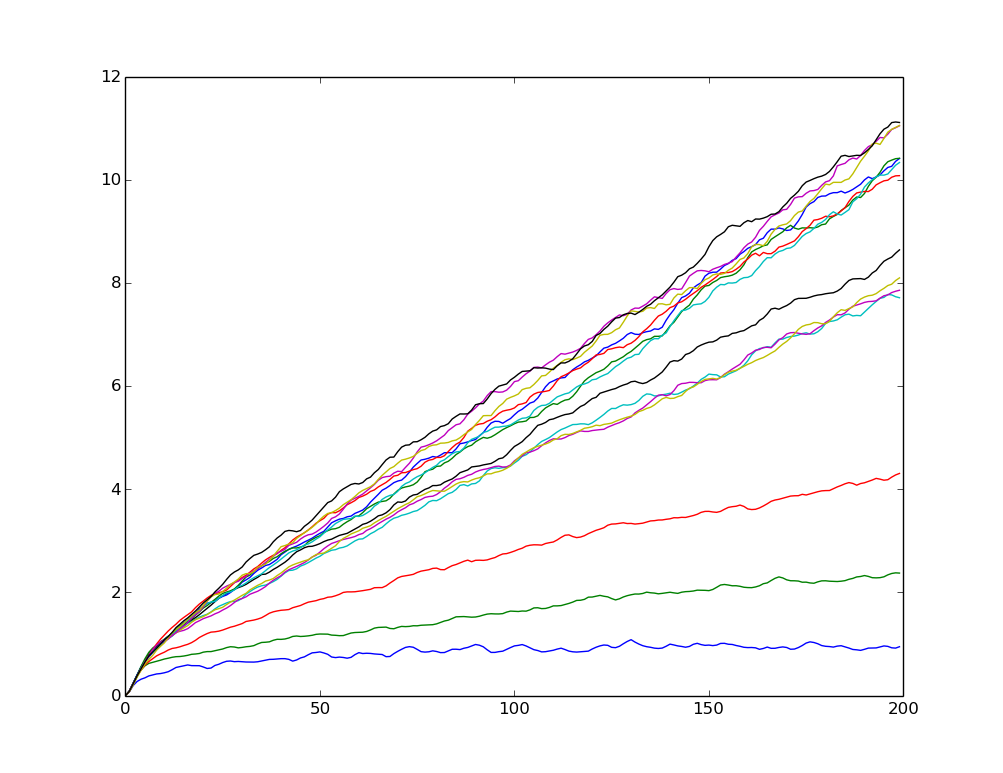
\includegraphics[width=0.5\textwidth]{images/diffusion/mean_square_displacement_interesting.png}%
%     \caption{%
%         Something interesting (msd stops increasing for a couple of angstrom near 4.5-5, 5-5.5, 5.5-6.0) \hl{reference figure or remove} \hl{FINISH CAPTION}. %
% %         \label{fig:cell_lists}%
%     }%
% \end{figure}%

% \begin{figure}[htpb]%
%     \centering%
%     \setlength{\myfigwidth}{0.49\textwidth}%
% %     \setlength{\mycaptionwidth}{0.3\textwidth}%
% %
%     \begin{subfigure}[b]{\myfigwidth}%
%         \includesvg[width=\textwidth, svgpath=./images/diffusion/]{diffusion_constant_move_origin01}%
%         \caption{%
%             Diffusion. \hl{FINISH CAPTION}. %
%     %         \label{fig:cell_lists}%
%         }%
%     \end{subfigure}%
%     \hfill%
%     \begin{subfigure}[b]{\myfigwidth}%
%         \includesvg[width=\textwidth, svgpath=./images/diffusion/]{diffusion_constant_move_origin02}%
%         \caption{%
%             Diffusion. \hl{FINISH CAPTION}. %
%     %         \label{fig:cell_lists}%
%         }%
%     \end{subfigure}%
%     \caption{%
%         rough\_fracture\_01\_abel - ``Rough fracture \#1'' \hl{Caption} %
%         \label{fig:renderings_rough_fracture01_abel}%
%     }%
% \end{figure}%
\FloatBarrier
\section{Tetrahedral order parameter}
% \todoa{Bin width 0.5 \AA\ and $\Delta Q = 0.01$ for all results! ($\Delta Q$ isn't shown anywhere)}
% \todoa{Make two separate TOP figures, one for regular rough, and one for rough with same surfac x2 ?}
% \todoa{Update bulk TOP figure with results from long analysis run}
% %
% \begin{figure}[htpb]%
%     \centering%
%     \includesvg[width=1.0\textwidth, svgpath = ./images/tetrahedral_order_parameter/]{fancyfig04}%
%     \caption{}%
% %     \label{fig:distance_to_atom_r20}%
% \end{figure}%
%
% \begin{figure}[htpb]%
%     \centering%
%     \includesvg[%
% %         width=\textwidth,% choose which fits best, width or height (regular includegraphics can use both and add "keepaspectratio", but includesvg can't)
%         height=\textheight,%
%         svgpath = ./images/tetrahedral_order_parameter_new/]{figure01}%
%     \caption{\hl{Caption, add legends!}}%
% %     \label{fig:distance_to_atom_r20}%
% \end{figure}%
%

We have measured the thetrahedral order parameter for our four reference systems, and the four random fracture systems, and plotted the \hl{relative occurrence/probability} $P(Q)$ as function of $Q$, for water molecules with different distances from the silica matrix. We used used 150 bins for the $Q$-values, with $\Delta Q = 0.01$, and bins of $\Delta r = 0.5$ for the different distances to the matrix, for all measurements presented here. The results are plotted in \crefrange{fig:first_top_figure}{fig:last_top_figure}. We have also measured the bulk order parameter, which is plotted in \cref{fig:top_bulk}.

For comparison we have also estimated $P(Q)$ in bulk water, by measuring the tetrahedral order parameter for all water molecules further from the silica matrix than 10 \AA, in the two reference systems with 86 \AA\ wide flat pores. The results for bulk water can be seen in \cref{fig:top_bulk}. We see that we get \hl{two peaks (``bimodal''?)}, one just above $Q = 0.5$ and one right below $Q = 0.75$. \todoao{Compare with some reference, for example Mathilde's ref [26]?}
%
\begin{figure}[htpb]%
    \centering% 
    \includesvg[%
        width=0.5\textwidth,
        svgpath = ./images/tetrahedral_order_parameter_new/%
    ]{figure01_bulk}%
    \caption{%
        Plot of tetrahedral order parameter for bulk water (water molecules further than 10 \AA\ from the silica matrix), in the two reference systems with 86 \AA\ wide flat pores (reference system \#1 and \#2, see \cref{fig:renderings_flat_square_fracture02,fig:renderings_flat_square_fracture03}). The average $Q$ is indicated by a vertical line. %
    }%
    \label{fig:top_bulk}%
\end{figure}%

In \cref{fig:top_normal_and_reference,fig:top_narrow01_and_reference,fig:top_narrow02_and_reference} we have plotted the results for different combinations of random fractures and flat pores. We have plotted this for a total of %
% 10 %
8 %
different distances from the silica matrix, for $Q$-values ranging from -0.5 to 1.0. 

We see that all systems have pretty similar behaviour for different $Q$-values, but we also see that $P(Q)$ changes a lot when we go from 3.0 \AA\ from the silica matrix to 5 \AA. At 5.5 \AA we are already pretty close to the bulk behaviour seen in \cref{fig:top_bulk}, with a small gradual change from 5.5 \AA\ to 6.5 \AA\ (and further to 10 \AA, not plotted here), where we are close to bulk behaviour. In general we see that near the silica matrix water seems to have a very different internal coordination compared to in bulk water, with the average $Q$-value going from $Q_\text{mean} \approx 0.2$ at $r = 3.0$ \AA\ to $Q_\text{mean} \approx 0.55$ at $r = 4.5$ \AA, in all systems, which is close to the bulk value of $Q_\text{mean, bulk} \approx 0.63$. We also see that the distribution has a different shape at $r = 4.5$ \AA\ than the bulk distribution. We also see that $P(Q)$ is much more spread out close to the silica matrix compared to further away, and that we only have a single peak, while bulk water has \hl{two peaks (``bimodal''?)} and is less spread out.\todobo{come up with something more accurate than ``spread out''}
\todob{Table of mean Q? Stddv?}

%
\begin{figure}[!p]%
    \centering%
    \includesvg[%
        width=\textwidth,% choose which fits best, width or height (regular includegraphics can use both and add "keepaspectratio", but includesvg can't)
%         height=\textheight,%
        svgpath = ./images/tetrahedral_order_parameter_new/%
    ]{figure02_regular_and_wide}%
    {%
        \captionsetup{width=\textwidth}%
        \caption{%
            Plot of $P(Q)$ for the two regular rough fractures (the solid lines), and a reference system with a 86 \AA\ wide flat pore (the dashed line) (see \cref{fig:renderings_rough_fracture01_abel,fig:renderings_rough_fracture03,fig:renderings_flat_square_fracture03}), for different distances to the silica matrix (as indicated by the text in top left corner of each plot). The average $Q$ is indicated by a vertical line. %
            \label{fig:top_normal_and_reference}%
            \label{fig:first_top_figure}%
        }%
    }%
\end{figure}%

In figure \cref{fig:top_normal_and_reference} we have plots of $P(Q)$ for rough systems \#1 and \#2, which are the two random rough fractures, and reference system \#1, which is a 86 \AA\ wide flat pore with a bulk water density of $\sim 1038$ kg/m$^3$. We see that the two random fracture systems have very similar behaviour, as expected, since they were prepared very similarly. We see that the average $Q$-value of the fracture systems is generally lower than in the reference system, and that the fracture systems seem to ``lag behind'' the reference system when we increase the distance to the silica matrix, with the fractured systems catching up the reference system near 6.5 \AA, as all three plots get close to a bulk-like shape.

%
\begin{figure}[!p]%
    \centering% 
    \includesvg[%
        width=\textwidth,% choose which fits best, width or height (regular includegraphics can use both and add "keepaspectratio", but includesvg can't)
%         height=\textheight,%
        svgpath = ./images/tetrahedral_order_parameter_new/%
    ]{figure02_flat_and_wide01}%
    {%
        \captionsetup{width=\textwidth}%
        \caption{%
            Plot of $P(Q)$ for a rough fracture with uniform width of 14.4 \AA\ (the blue solid line), a reference system with a 14.4 \AA\ wide flat pore (the dashed line), and a flat reference system with a 86 \AA\ wide flat pore (the red solid line) (see \cref{fig:renderings_rough_fracture04_same_distance,fig:renderings_flat_fracture03,fig:renderings_flat_square_fracture03}), for different distances to the silica matrix (as indicated by the text in top left corner of each plot). The average $Q$ is indicated by a vertical line. %
            \label{fig:top_narrow01_and_reference}%
        }%
    }%
\end{figure}%

In \cref{fig:top_narrow01_and_reference} we have plots of $P(Q)$ for rough system \#3, which is the fracture with uniform width of 14.4 \AA, and reference systems \#1 and \#3, which are the 86 and 14.4 \AA\ wide flat pores. %
We see that that the reference system with a wide flat pore seems to lie between the two systems with narrow pores for $r\in[3.5,5.5]$, and that the narrow fracture seems to lag behind the two reference systems as we increase $r$ from 3.5 to 6.0 \AA, with the behaviour in all systems being close to bulk at $6.0$ \AA. We see that the average $Q$ for the narrow fracture seems to lie lower than the wide flat pore reference system, and the narrow flat pore reference system seems to lie higher.
% We see the same trend in $P(Q)$ as before, with the average $Q$ being lower for the fracture and the narrow flat pore for $r < 5.5$ \AA, and the shape of $P(Q)$ getting close to bulk as $r\rightarrow 6.0$ \AA. We see that $P(Q)$ for the narrow flat pore seems to lie between the narrow fracture and the reference system, and that both the narrow fracture and narrow pore seems to lag behind the reference system as we increase the distance to the silic matrix.

%
\begin{figure}[!p]%
    \centering% 
    \includesvg[%
        width=\textwidth,% choose which fits best, width or height (regular includegraphics can use both and add "keepaspectratio", but includesvg can't)
%         height=\textheight,%
        svgpath = ./images/tetrahedral_order_parameter_new/%
    ]{figure02_flat_and_wide02}%
    {%
        \captionsetup{width=\textwidth}%
        \caption{%
            Plot of $P(Q)$ for a rough fracture with uniform width of 28.8 \AA\ (the blue solid line), a reference system with a 28.8 \AA\ wide flat pore (the dashed line), and a reference system with a 86 \AA\ wide flat pore (the red solid line) (see \cref{fig:renderings_rough_fracture05,fig:renderings_flat_fracture03,fig:renderings_flat_square_fracture03}), for different distances to the silica matrix (as indicated by the text in top left corner of each plot). The average $Q$ is indicated by a vertical line. %
            \label{fig:top_narrow02_and_reference}%
        }%
    }%
\end{figure}%

In \cref{fig:top_narrow01_and_reference} we have plots of $P(Q)$ for rough system \#4, which is the fracture with uniform width of 28.8 \AA, and reference systems \#1 and \#4, which are the 86 and 28.8 \AA\ wide flat pores. We see the same behaviour as for the 14.4 \AA\ fracture, albeit with the 28.8 \AA\ reference system being a bit closer to the reference system with a wide fracture.

In both \cref{fig:top_narrow01_and_reference,fig:top_narrow02_and_reference} it seems like the systems with a narrow flat pore (the red solid lines) seems to deviate the most from the wide reference system.

%
\begin{figure}[htpb]%
    \centering% 
    \includesvg[%
        width=\textwidth,% choose which fits best, width or height (regular includegraphics can use both and add "keepaspectratio", but includesvg can't)
%         height=\textheight,%
        svgpath = ./images/tetrahedral_order_parameter_new/%
    ]{figure02_all_rough}%
    {%
%         \captionsetup{width=\textwidth}%
        \caption{%
            \hl{Caption} %
            \label{fig:top_all_rough_and_one_reference}%
            \label{fig:last_top_figure}%
        }%
    }%
\end{figure}%

In \cref{fig:top_all_rough_and_one_reference} we have plotted $P(Q)$ for all rough fracture systems and reference \#1, which is the 86 \AA\ wide flat fracture. We see that the average $Q$ for all fracture systems seems to lie below the reference system, and they all seem to lag beind the reference system as we increase $r$ from 3.5 to 5.5 \AA.
\FloatBarrier
\section{Distance to nearest atom}
% \todoa{Mention that images are made with no water molecules (only passivation atoms) in system}
%
We have made 3d maps of the system labelled ``rough fracture \#2'', using the method from \cref{sec:distance_to_atom}, which finds the distance to the nearest atom on a grid of points. The results can be seen in \cref{fig:distance_to_atom_r05,fig:distance_to_atom_r20}, where we show slices of the maps in the $yz$- and $xy$-plane. For the first figure we used a max distance of 5 \AA, while for the second one we used a max distance of 20 \AA. The maps were made from the molecular system after cutting out the atoms to make the pore and passivating the dangling ends, but before filling the pore with water. A similar map can me made by not including the water molecules in the calculations.

In \cref{fig:distance_to_atom_r05} we can clearly see the positions of the atoms in the silica matrix as the dark blue dots, while the pores light up as red areas.

In \cref{fig:distance_to_atom_r20} we still see the positions of the atoms, but they are less visible now since we have a bigger range for the colormap. We can still see the pores easily, colored white, and we now also see some characteristics of the pore itself, where it has a darker red color.%
%
\begin{figure}[htpb]%
    \centering%
    \setlength{\myfigwidth}{0.9\textwidth}%
    \begin{subfigure}[b]{\myfigwidth}%
        \includesvg[pretex=\normalsize, width=\textwidth, svgpath = ./images/distance_to_atom/rough_fracture_03/]{05_r05_n256}%
        \caption{Max distance $r_\text{max}=5.0$ \AA.%
        \label{fig:distance_to_atom_r05}}%
    \end{subfigure}%
    \vspace{10pt}
    \begin{subfigure}[b]{\myfigwidth}%
        \includesvg[pretex=\normalsize, width=\textwidth, svgpath = ./images/distance_to_atom/rough_fracture_03/]{05_r20_n256}%
        \caption{Max distance $r_\text{max}=20$ \AA.%
        \label{fig:distance_to_atom_r20}}%
    \end{subfigure}%
    \caption{%
        Slices of 3d maps of the distance to the nearest atom in the system labelled ``rough fracture \#2'', generated using method from \cref{sec:distance_to_atom}, using a colormap that goes from \textbf{(a)} 0 to 5 \AA, and \textbf{(b)} 0 to 20 \AA.%
    }%
\end{figure}%
% \FloatBarrier
\section{``Generation matrix''}
\todo{replace these with results from actual fracture system?}
Not very useful. Much of the same as distance to atom, only worse (but faster). Quantitatively much the same as distance to atom?
%
\setlength{\myfigwidth}{0.90\textwidth}%
\begin{figure}[htpb]%
    \centering%
    \includesvg[pretex=\normalsize, width=\myfigwidth, svgpath = ./images/generation_matrix/rough_fracture03/]{05_r0745_n256}%
    \caption{7.45 generations, Manhattan distance of $\sim 5$ \AA.}%
    \label{fig:generation_matrix_r05}%
\end{figure}%
%
\begin{figure}[htpb]%
    \centering%
    \includesvg[pretex=\normalsize, width=\myfigwidth, svgpath = ./images/generation_matrix/rough_fracture03/]{05_r308_n256}%
    \caption{30.8 generations, Manhattan distance of $\sim 20$ \AA \hl{really 20.7 because I used 30.8 instead of 29.8 generations....}.}%
    \label{fig:generation_matrix_r11}%
\end{figure}%
% %
% \begin{figure}[htpb]%
%     \centering%
%     \includesvg[pretex=\normalsize, width=\myfigwidth, svgpath = ./images/generation_matrix/]{SiO2_06_slice_r40_n256}%
%     \caption{40 generations}%
%     \label{fig:generation_matrix_r40}%
% \end{figure}%
\FloatBarrier

% \section{Area}
% \section{Volume?}

